\chapter{Coil array WPT}\chaplab{result}
% 通过上一章节的讲解,我们知道了无线传输系统在水下的基本表现。这章将介绍我们设计出的水下线圈组wpt系统,通过将大型的双线圈结构降解为多个小线圈结构,这使得内部线圈里面的磁场大幅减小,从而实现对AUV系统内部的电磁保护。
Through the explanation in the previous chapter, we know the basic performance of the wireless transmission system underwater. This chapter will introduce the underwater coil-array WPT system we designed, by degrading a large double coil structure into multiple small coil structures, as shown in figure \ref{fig:3_coil_array_structure}. This greatly reduces the magnetic field in the internal coil, thereby achieving electromagnetic protection inside the AUV system. Its detailed parameters are shown in table \ref{table: coil array parameters}.

\begin{figure}[!b]
    \centering
    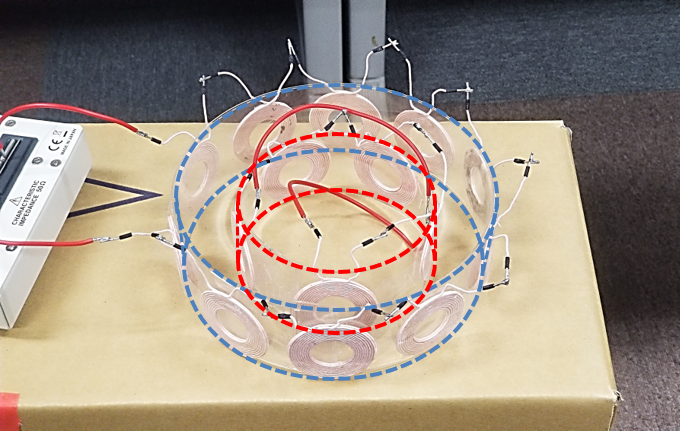
\includegraphics[width=0.7\linewidth]{images/3_coil_array_structure.png}
    \caption{Coil-array structure.}
    \label{fig:3_coil_array_structure}
\end{figure}

% 参数表格
\begin{table}[!t]
    \centering
    \caption{The parameters of coil-array structure.}
    \begin{tabular}{ c|cc }
        \thickhline
        % \hline
        \textbf{Items}         & \textbf{Parameters}      \\
        \thickhline
        Tx coil diameter       & 160mm                    \\ \hline
        Rx coil diameter       & 100mm                     \\ \hline
        The number of Tx coils & 10                       \\ \hline
        The number of Rx coils & 5                        \\ \hline
        Coil connection        & In series                \\ \hline
        Coil model             & WE 760308110 (Litz wire) \\ \hline
    \end{tabular}
    \label{table: coil array parameters}
\end{table}

In the marine environment, we can use buoys to generate electricity \cite{Orekan}, store the collected electricity in the power source, and then connect the power source to the transmitter (Tx). When the AUV (Rx) reaches the designated position of the transmitter, the AUV can be charged wirelessly. This is the basic workflow of this UWPT system.
Figure \ref{fig:3_coil_array_uwpt} shows a schematic diagram of the UWPT system.

\begin{figure}[!t]
    \centering
    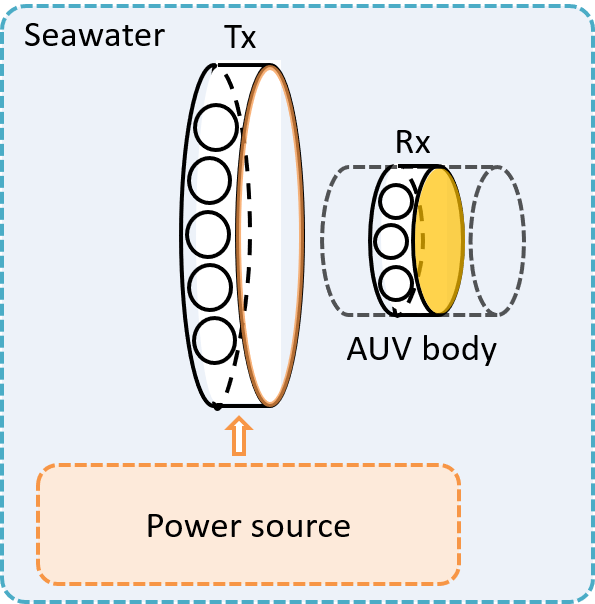
\includegraphics[width=0.5\linewidth]{images/3_coil_array_uwpt.png}
    \caption{Sechematic diagram of coil-array UWPT system.}
    \label{fig:3_coil_array_uwpt}
\end{figure}
In the following subsections, the performance of the coil-array UWPT system will be described in detail.


\section{Measurement of the coil-array WPT system}

In this section, we will first introduce different coil arrangements. By changing the coil structure of the coil-array, observe the performance of the changed coil structure under different conditions.

As shown in figure \ref{fig: 10-5 with ferrite}, a transmitter coil with a radius of 80mm is used here, which consists of 10 coils with ferrite in series, and a receiver coil with a radius of 50mm, which consists of 5 coils with ferrite in series. Therefore, the distance between Tx and Rx is 30mm. For other specific parameters, please find in the figure \ref{fig: 10-5 with ferrite}.

\begin{figure}[!t]
    \centering
    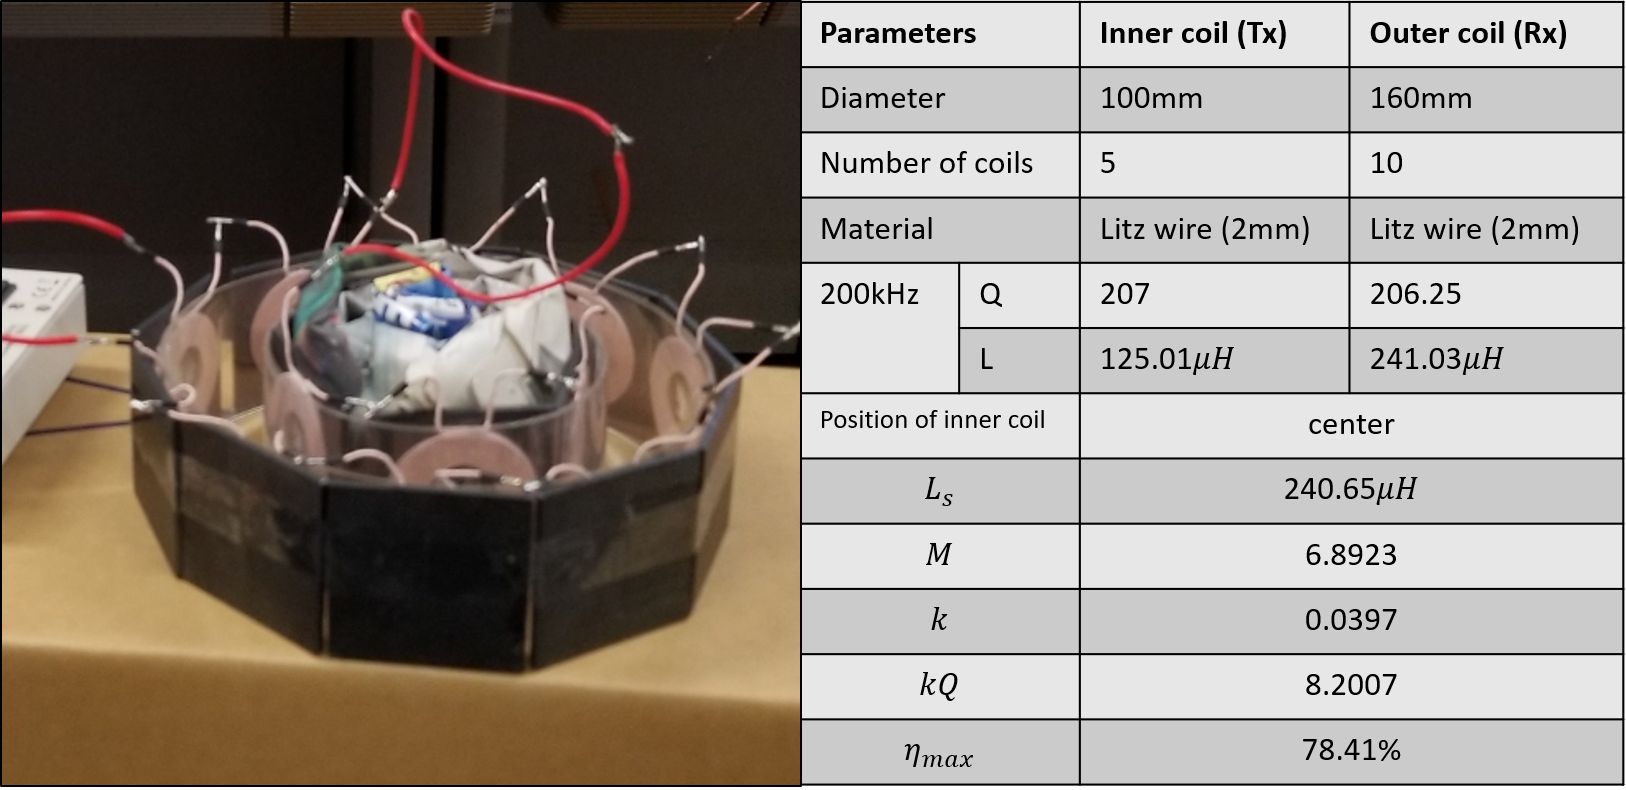
\includegraphics[width=1.0\linewidth]{images/4_coil_5_10_with_ferrite.png}
    \caption{Coil-array IPT structure (Both sides with ferrite tile), inner coil in the center or the outer coil.}
    \label{fig: 10-5 with ferrite}
\end{figure}
By using LCR meter to measure this arrangement system, we can get the inductance of the Tx's coil-array coil, $L_1 = 241.03 \mu H$, and quality factor $Q_1=206.25$. And the inductance of Rx's coil-array coil, $L_2 = 125.01 \mu H$, and quality factor $Q_2=207$. Then short-circuit the Rx coil and place it in the middle of the Tx coil, and measure the inductance of the Tx in this state (As shown in figure \ref{fig: Ls}), which is $L_s$, where $L_s = 240.65 \mu H$.

\begin{figure}[!b]
    \centering
    % 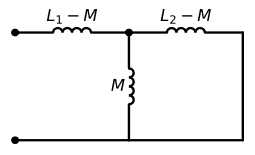
\includegraphics{images/3_mutual_inductance.png}
    \begin{tikzpicture}[scale=1, every node/.style={scale=1}, american voltages]
        \draw
        (1.5,3.5)
        to [short, o-] (4,3.5)
        to [L, l=$L_1$] (4,0)
        to [short, -o] (1.5,0);
        %\draw(-0.5,3.5) to [L,l=$M$] (-0.5,0);
        
        \draw
        (6,3.5) to [L, l_=$L_2$, mirror] (6,0)
        to [short, -o] (8.5,0)   ;
        \draw (8.5,3.5) to [short, o-]  (6,3.5);

        % source
        \node[below] at (5,3.5) {$M$};
        \draw [{<->}](4.234,2.6428) arc (139.9978:40:1);
    \end{tikzpicture}
    \caption{Measurement of $L_s$.}
    \label{fig: Ls}
\end{figure}

\begin{figure}[!t]
    \centering
    % 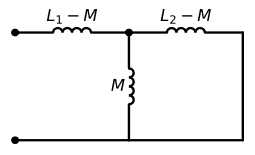
\includegraphics{images/3_mutual_inductance.png}
    \begin{tikzpicture}[scale=1, every node/.style={scale=1}, american voltages]
        \draw
        (0.75,2.75)
        to [L,l=$L_1-M$, *-] (4.5,2.75)
        to [L, l=$M$] (4.5,-1)
        to [short, -*] (0.75,-1);
        \draw
        (8.25,2.75) to [short] (8.25,-1)
        to [short] (4.5,-1)   ;
        \draw (4.5,2.75) to [L,l=$L_2-M$]  (8.25,2.75);
    \end{tikzpicture}
    \caption{Equivalent circuit of two coil model.}
    \label{fig: Ls eq}
\end{figure}

From equivalent circuit (Figure \ref{fig: Ls eq}), we can get the following formula.
\begin{equation}
    L_s = L_1 - M + \frac{M(L_2 - M)}{L_2}.
\end{equation}

Move $M$ to the left side of the equation, the mutual inductance can be expressed as,
\begin{equation}
    M = \sqrt{L_2(L_1-L_s)},
\end{equation}
and coupling coefficient,
\begin{equation}
    k = \frac{M}{L_1L_2}.
\end{equation}
$kQ$ pruduct can be expressed as,
\begin{equation}
    kQ = k\sqrt{Q_1Q_2}.
\end{equation}
$kQ$ product is an index showing the performance of a wireless transfer. The relationship between the maximum transmission efficiency $\eta_{max}$ and $kQ$ as follows \cite{Li2015, Ohira2014},
\begin{equation}
    \eta_{max} = \frac{k^2Q_1Q_2}{(1+\sqrt{1+k^2Q_1Q_2})^2}.
\end{equation}
According to the calculation of the above formula, we can get that the maximum transmission efficiency $\eta_{max}$ of this arrangement is $78.41\%$.

\section{The other coil arrangements and comparison}
% 接下来,我们通过增加线圈个数,改变Rx线圈在Tx线圈中的位置,来观察不同条件下系统的表现。结果如下图()所示。
Next, we will observe the performance of the system under different conditions by increasing the number of coils and changing the position of the Rx coil in the Tx coil. The result is shown in the figure \ref{fig: coil-array result1}, figure \ref{fig: coil-array result2}, and figure \ref{fig: coil-array result3}.
\begin{figure}[!b]
    \centering
    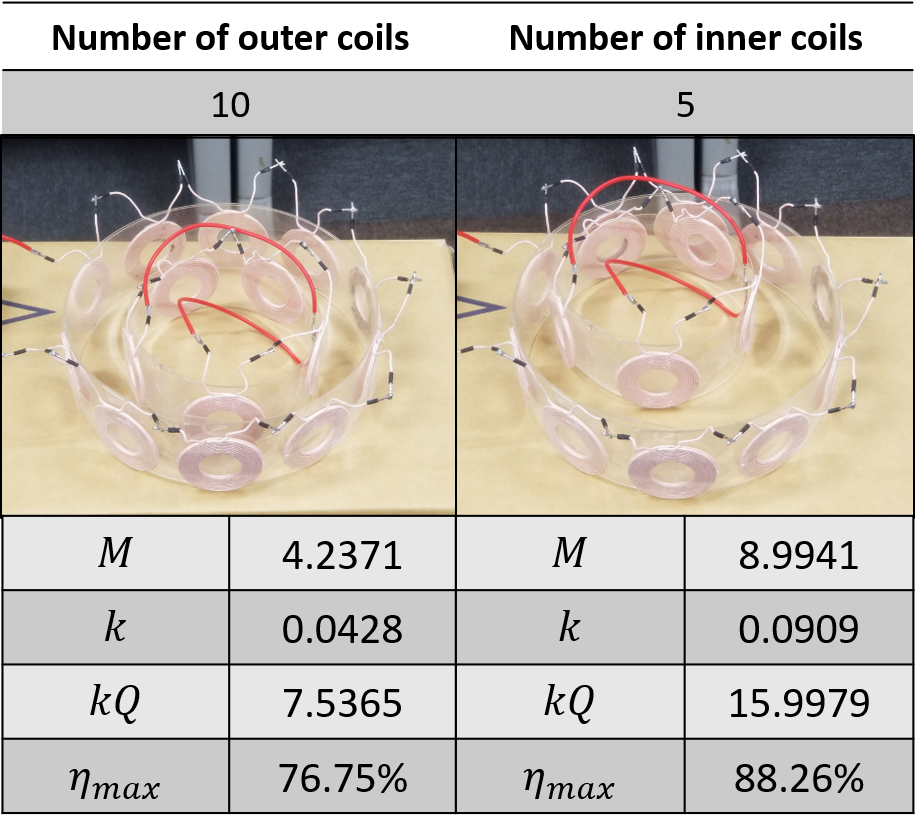
\includegraphics[width=0.65\textwidth]{images/4_coil_5_10_without_ferrite.png}
    \caption{Coil-array IPT structure (Both sides without ferrite tile), inner coil in the center of the outer coil (Left), inner coil next to the outer coil (Right).}
    \label{fig: coil-array result1}
\end{figure}
\begin{figure}[!t]
    \centering
    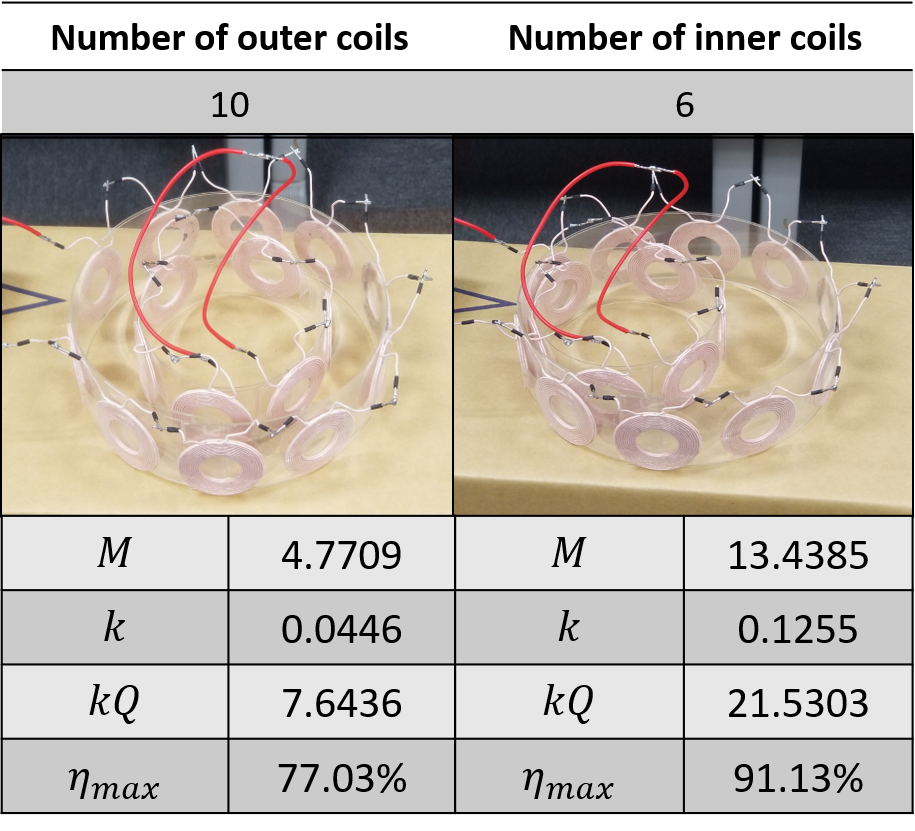
\includegraphics[width=0.65\textwidth]{images/4_coil_6_10_without_ferrite.png}
    \caption{Coil-array IPT structure (Both sides without ferrite tile), inner coil in the center of the outer coil (Left), inner coil next to the outer coil (Right).}
    \label{fig: coil-array result2}
\end{figure}
\begin{figure}[!t]
    \centering
    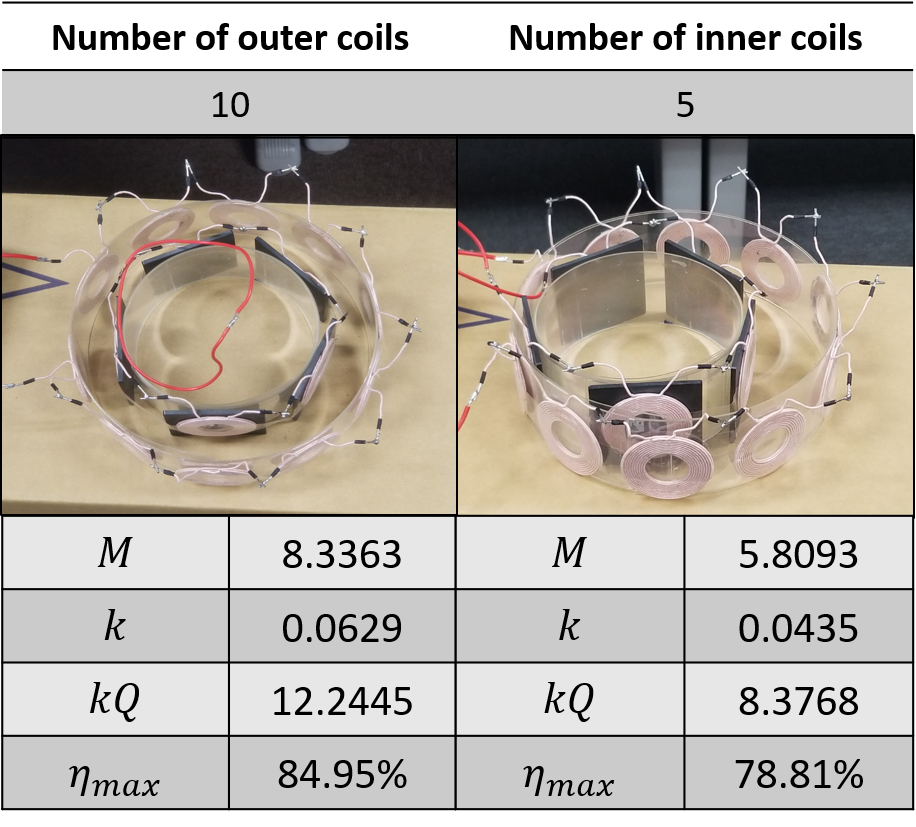
\includegraphics[width=0.65\textwidth]{images/4_coil_6_10_inner_with_ferrite.png}
    \caption{Coil-array IPT structure (Inner small coils with ferrite tile, outer small coils without ferrite tile), inner coil in the center of the outer coil (Left), inner coil next to the outer coil (Right).}
    \label{fig: coil-array result3}
\end{figure}


\begin{table}[!b]
    \centering
    \caption{Maximum power transfer efficiency of different coil arrangements.}
    \resizebox*{\textwidth}{!}{
    \begin{tabular}{|>{\centering\arraybackslash}m{3.3cm}|>{\centering\arraybackslash}m{2.5cm}|>{\centering\arraybackslash}m{2.5cm}|>{\centering\arraybackslash}m{2.5cm}|>{\centering\arraybackslash}m{2.5cm}|}
        \hline
        \textbf{Shift}                                        & \textbf{Numbers of coil (Outer - Inner)} & \textbf{Both coils with ferrite} & \textbf{Both coils without ferrite} & \textbf{Outer coils without ferrite, inner coils with ferrite} \\ \hline
        \multirow{2}{3.3cm}{Inner coil in the center}         & 10 - 5                                   & 78.41\%                          & 76.75\%                             & 84.95\%                                                        \\ \cline{2-5}
                                                              & 10 - 6                                   &                                  & 77.03\%                             &                                                                \\ \hline
        \multirow{2}{3.3cm}{Inner coil close to the one side} & 10 - 5                                   &                                  & 88.26\%                             & 78.80\%                                                        \\ \cline{2-5}
                                                              & 10 - 6                                   &                                  & 91.13\%                             &                                                                \\ \hline
    \end{tabular}}
    \label{table: comparison of the different coil arrangement}
\end{table}

% 通过上面各个方案下的结果,我们可以将其汇总成表1,如下
Through the results under each of the above scenarios, we can summarize them into table \ref{table: comparison of the different coil arrangement}, as follows

From table \ref{table: comparison of the different coil arrangement}, we can get the following conclusions:
\begin{itemize}
    \item When we increase the number of inner coils, the maximum PTE (Power transfer efficiency) will increase.
    \item If the numbers of outer and inner coils are the same, when outer coils without ferrite and inner coils with ferrite, we can get the maximum PTE.
    \item When there is no ferrite outside the inner coil, the PTE will increase if the inner coil deviates from the middle, and vice versa.
\end{itemize}

\section{Megnetic field distribution}
% 为了弄清coil-array结构的磁场分布,我们使用了Wipl-d电磁模拟软件。我们对以下两个结构进行了模拟,具体参数如下表。
In order to clarify the magnetic field distribution of the coil-array structure, we used Wipl-d electromagnetic simulation software. We simulated the following two structures, and the specific parameters are as follows.

\begin{figure}[!t]
    \resizebox*{\textwidth}{!}{
    \begin{subfigure}{0.5\textwidth}
        \centering
        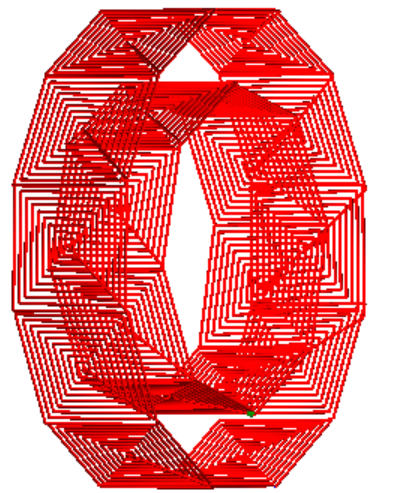
\includegraphics[height=6.4cm]{images/4_coil_array_system.png}
        \caption{Coil-array IPT structure.}
        \label{fig:subim1}
    \end{subfigure}
    \begin{subfigure}{0.5\textwidth}
        \centering
        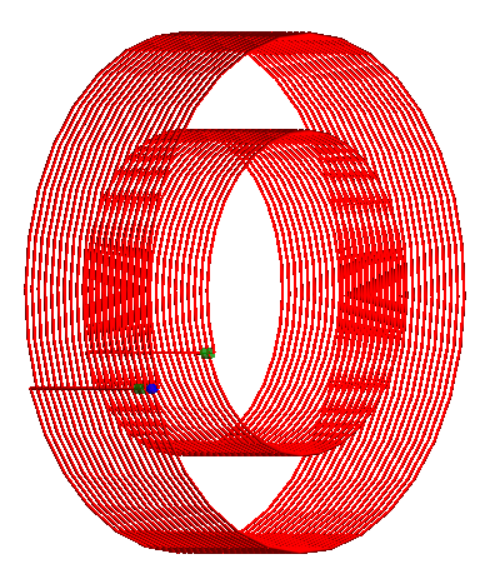
\includegraphics[height=6.4cm]{images/4_two_ring_system.png}
        \caption{Two ring IPT structure.}
        \label{fig:subim2}
    \end{subfigure}
    }
    \caption{Two kind of UWPT coil structure simulation diagram.}
    \label{fig:3_two_ring_coil}
\end{figure}
% 因此,我们得到了两种线圈结构的磁场分布图,如下
Therefore, we have obtained the magnetic field distribution diagrams of the two coil structures, as follows,

\begin{figure}[!t]
    \centering
    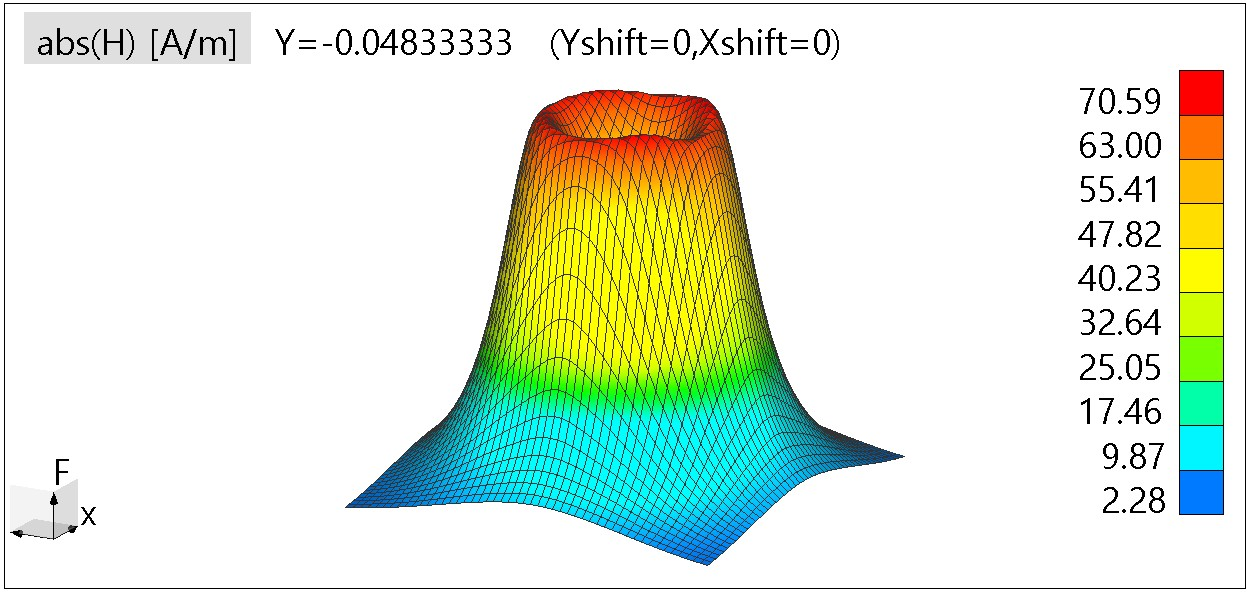
\includegraphics[width=0.9\linewidth]{images/4_coil_array_near_field_distribution.JPG}
    \caption{Magnetic field distribution of coil-array IPT structure.}
\end{figure}

\begin{figure}[!t]
    \centering
    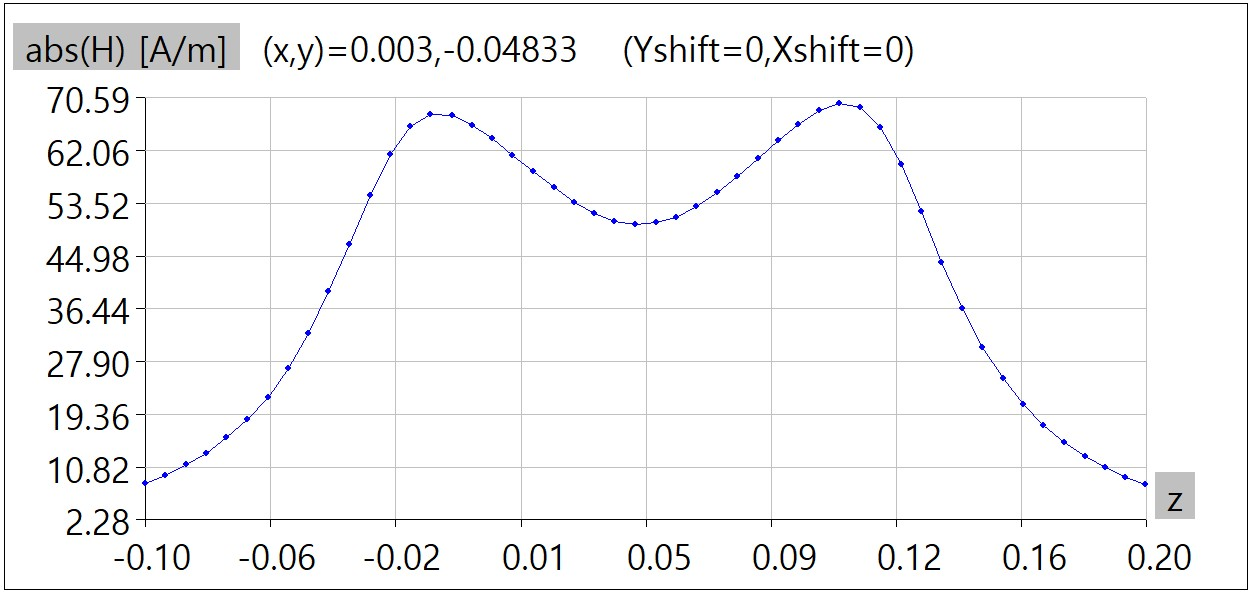
\includegraphics[width=0.9\linewidth]{images/4_coil_array_near_field_distribution_cut.JPG}
    \caption{Cross-sectional view of the magnetic field distribution of aoil-array IPT structure.}
\end{figure}

\begin{figure}[!t]
    \centering
    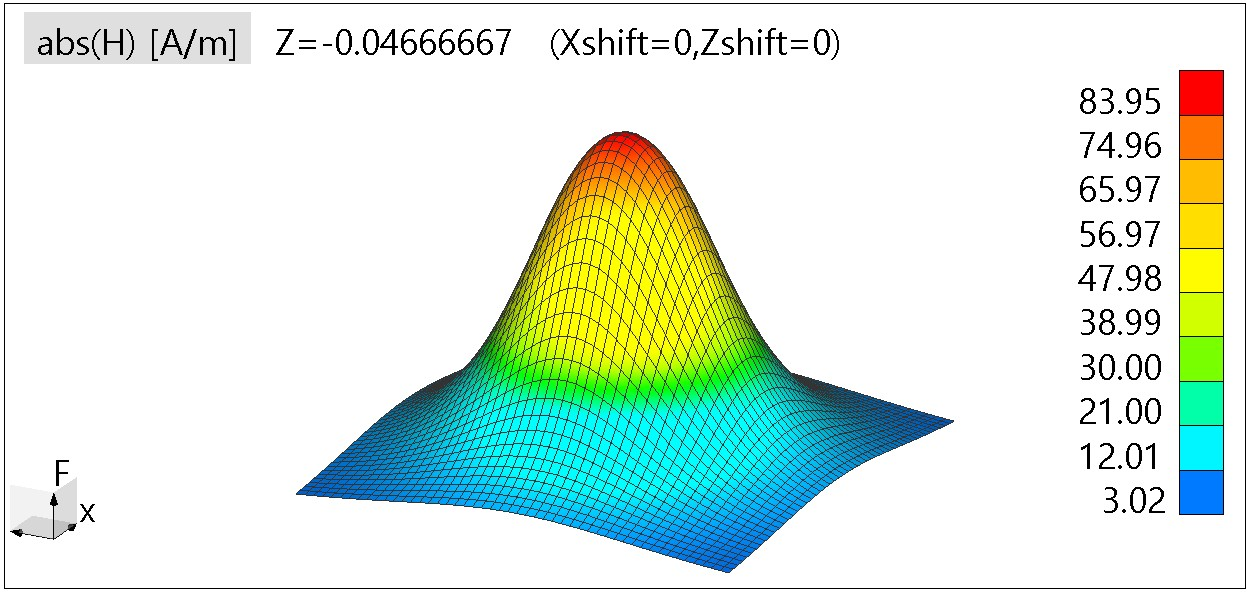
\includegraphics[width=0.9\linewidth]{images/4_two_ring_near_field_distribution.JPG}
    \caption{Magnetic field distribution of two ring IPT structure.}
\end{figure}

\begin{figure}[!t]
    \centering
    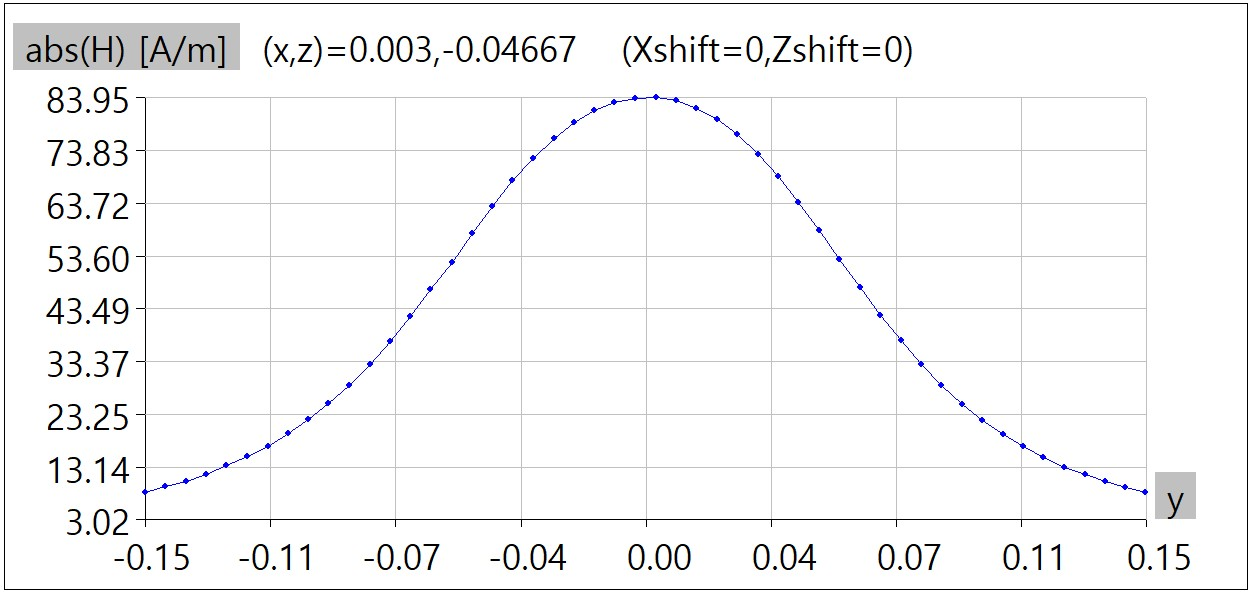
\includegraphics[width=0.9\linewidth]{images/4_two_ring_near_field_distribution_cut.JPG}
    \caption{Cross-sectional view o f the magnetic field distribution of two ring IPT structure.}
\end{figure}

% 我们可以发现当coil-array结构的中间磁场分布明显比two-ring结构要低。
% 改变内部线圈的偏移,双方向下的偏移。


\section{Coil array WPT under seawater}

